\documentclass[a4paper]{article}

\usepackage{../inc/ssarticle}
\title{{\centering\huge {Agentes auto-propulsados: Boids}}}

\begin{document}
\begin{titlingpage}
    \maketitle
    \begin{abstract}
        En el presente informe, se realiza un estudio del comportamiento de bandadas de agentes autopropulsados mediante la implementación y análisis del paper propuesto por Reynolds, C. W. \cite{BoidsPaper}.
    \end{abstract}
\end{titlingpage}

    \tableofcontents
    \newpage

    \section{Fundamentos}
        \subsection{Boids: Reglas}
            \begin{table}[h]
            \begin{tabular}{ccc}
                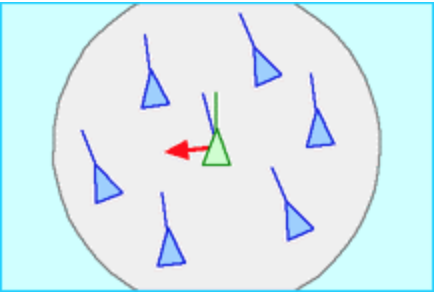
\includegraphics[width=0.3\linewidth]{{../imgs/rule_alignment}.png} &
                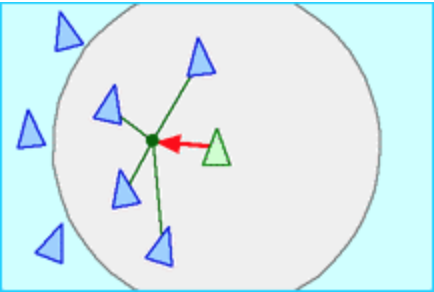
\includegraphics[width=0.3\linewidth]{{../imgs/rule_cohesion}.png} &
                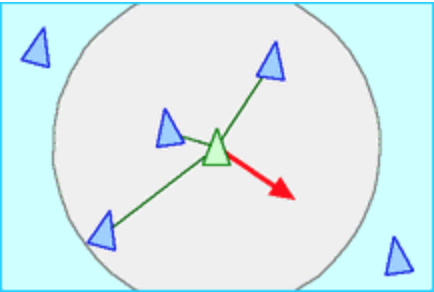
\includegraphics[width=0.3\linewidth]{{../imgs/rule_separation}.png} \\
                Alineamiento & Cohesión & Separación \\
            \end{tabular}
            \end{table}
        \subsection{Polarización}
            Se siguen los pasos de \textit{Vicsek et al.} y se calcula la polarización de la siguiente manera:

            \begin{equation} % Cálculo de la velocidad promedio
            v_a = \frac{1}{Nv}\left|\sum_{i=1}^{N}\mathbf{v}_i\right|
            \end{equation}

            donde $N$ es la cantidad de agentes en el universo, $v$ es la magnitud de la velocidad (igual para todos los agentes) y $\mathbf{v}_i$ es la velocidad de cada agente.

            La polarización nos permite tener un indicador sobre el estado del alineamiento de los agentes dentro del universo, en donde $0$ es desorden absoluto y $1$ es alineamiento perfecto (todos los agentes se mueven en exactamente la misma dirección).


        \subsection{Cálculo de vecinos}
            Para el cáclulo de vecinos se utiliza el método llamado \textit{Cell Index Method}. El mismo consiste en subdividir el espacio de simulación (Universo) en celdas cuadradas de un determinado largo de manera tal que el radio de búsqueda de vecinos sea menor que el largo de cada celda. Debido a que cada agente pertenece a una única celda y a que el ancho de la celda es mayor al radio de búsqueda, el método permite reducir el costo de búsqueda de vecinos de $N^2$ a $N$.


    \section{Implementación}

        \subsection{Universe}

            El universo utilizado para realizar la simulación es un hiperrectánculo con un largo $W$, alto $H$ y profundidad $D$. A su vez, es posible crear simulaciones con o sin condiciones de contorno.

            El universo, una vez creado, no puede ser modificado (ni sus dimensiones, ni parámetros, ni entidades), por lo que al avanzar la simulación, se van creando fotos del universo para cada tiempo específico.


            \begin{figure}[H]
                \centering
                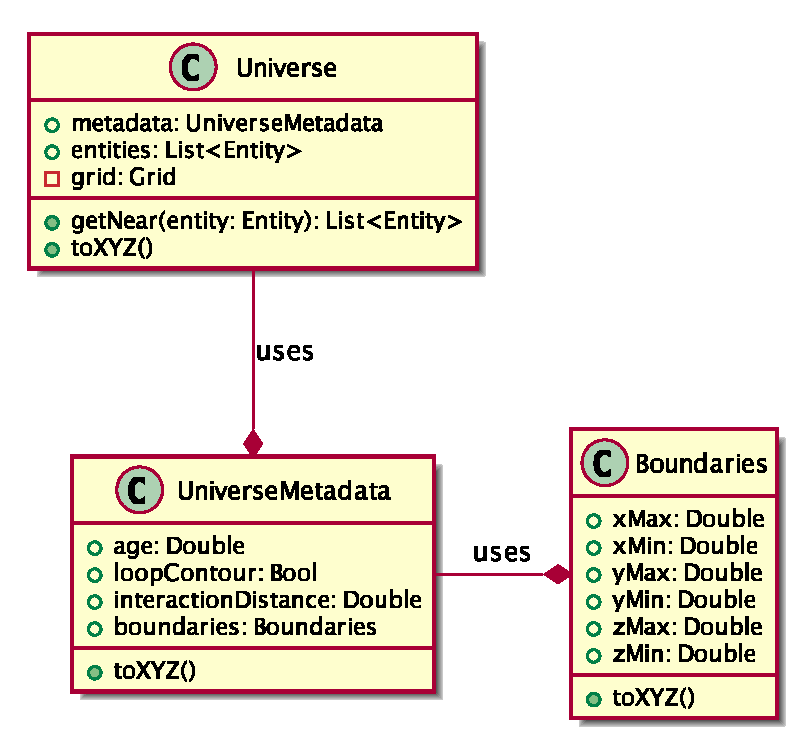
\includegraphics[width=0.5\textwidth]{../imgs/universe}
                \caption{Universo}
                \label{fig:universe_implementation}
            \end{figure}

        \subsection{Grid}

            \begin{figure}[H]
                \centering
                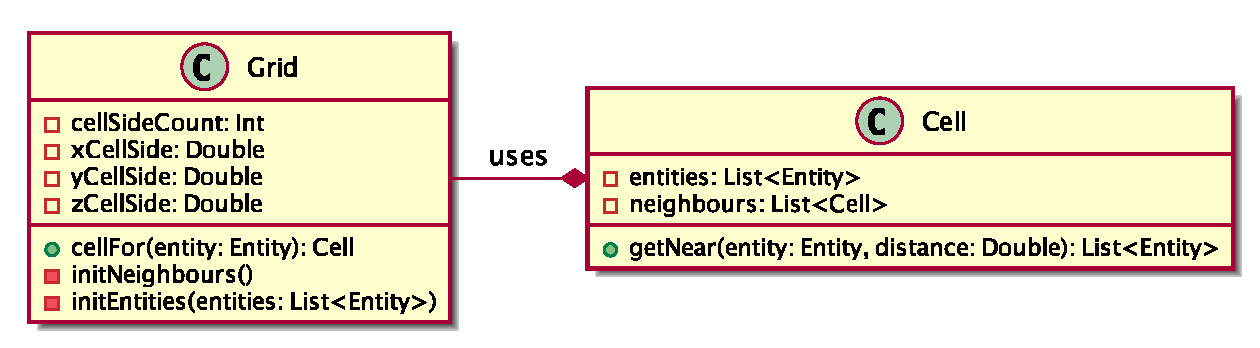
\includegraphics[width=0.8\textwidth]{../imgs/grid}
                \caption{Grilla}
                \label{fig:grid_implementation}
            \end{figure}

        \subsection{Entity}

            Cada agente es representado como un punto sin volumen. Está ubicado en un cierto punto del universo ($x, y$), comparte la misma magnitud de velocidad con el resto de los agentes pero cada uno tiene su própio ángulo.

            \begin{figure}[H]
                \centering
                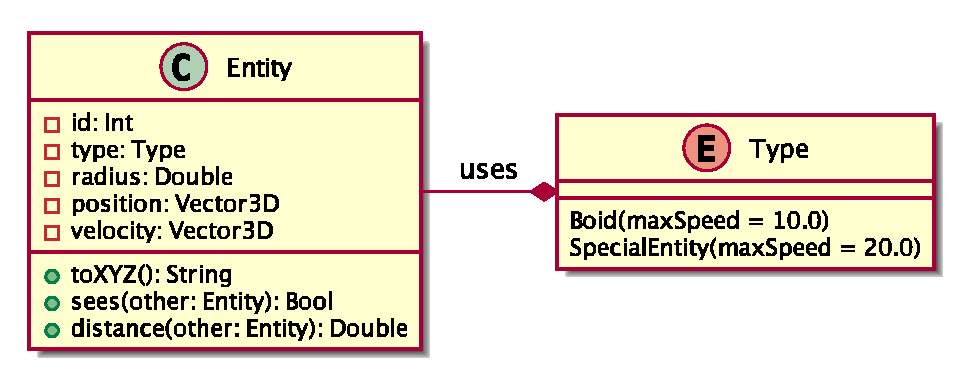
\includegraphics[width=0.5\textwidth]{../imgs/entity}
                \caption{Entidad}
                \label{fig:entity_implementation}
            \end{figure}

        \subsection{Rule}

            \begin{figure}[H]
                \centering
                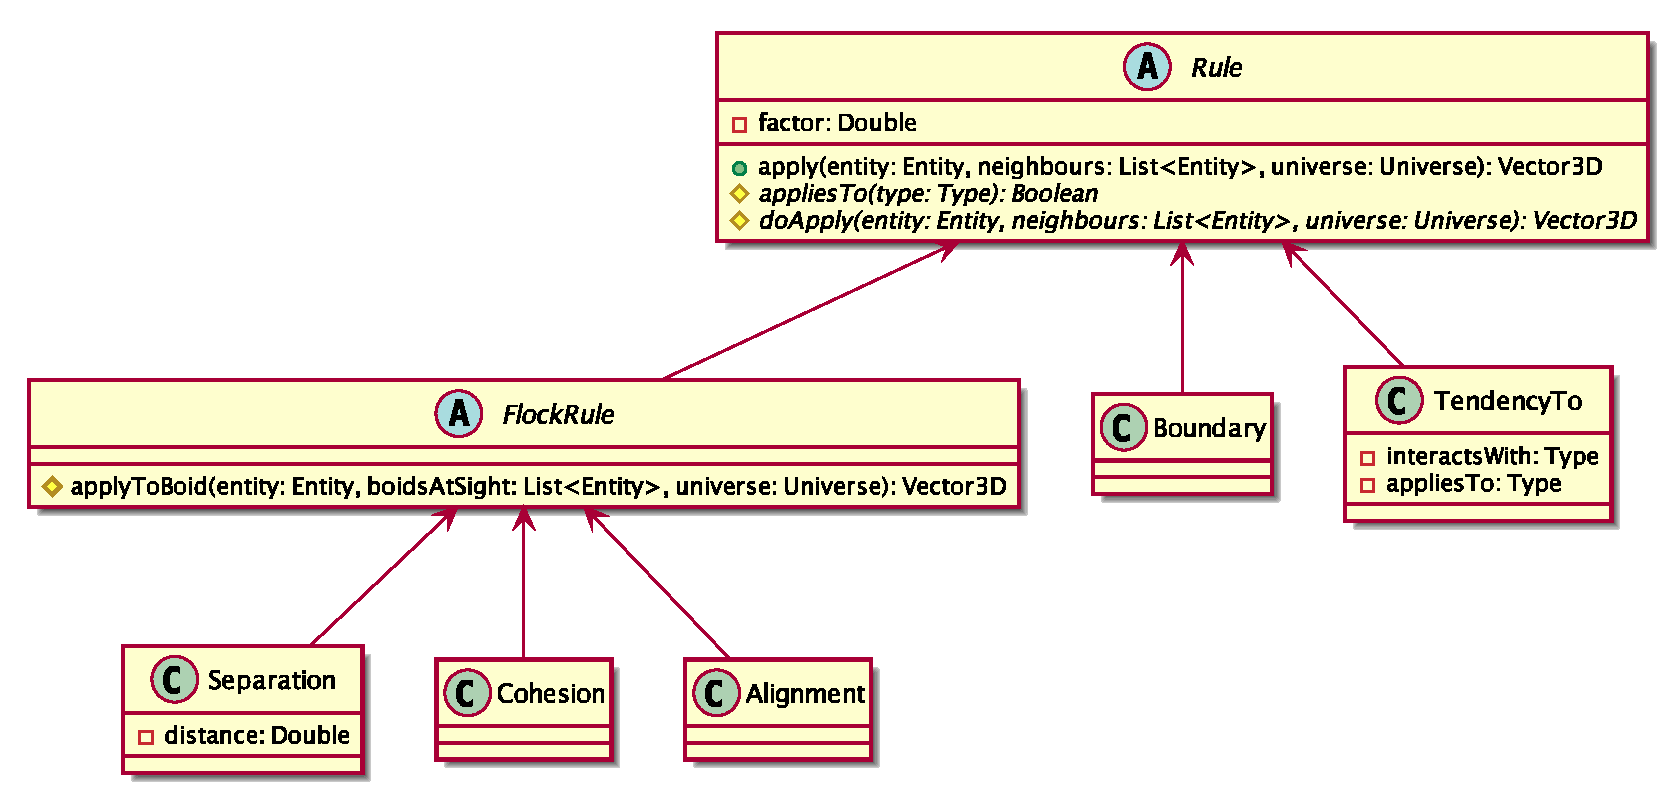
\includegraphics[width=0.8\textwidth]{../imgs/rules}
                \caption{Reglas}
                \label{fig:rules_implementation}
            \end{figure}
        \subsection{Simulation}

            \begin{figure}[H]
                \centering
                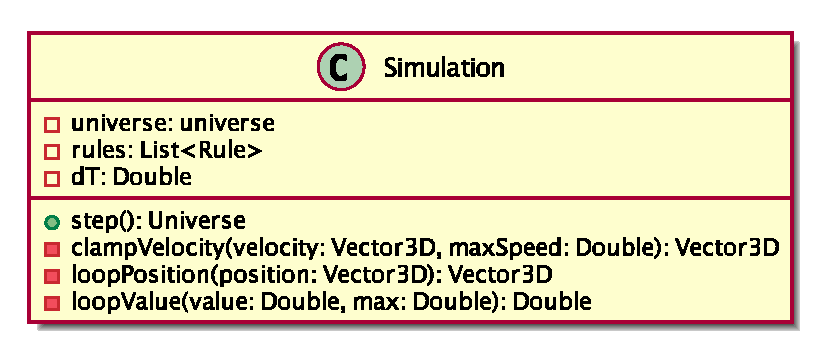
\includegraphics[width=0.5\textwidth]{../imgs/simulation}
                \caption{Simulación}
                \label{fig:simulation_implementation}
            \end{figure}

        \subsection{Simulación de agentes autopropulsados}

            Con los modelos anteriores, la simulación se realiza siguiendo la propuesta de \textit{Vicsek et al.} \cite{BoidsPaper} de manera tal que todos los agentes tienen una velocidad con la misma magnitud y cada uno se crea con un ángulo elegido al azar. Debido a la discretización del tiempo, la posición de cada agente se calcula de la siguiente manera:

            \begin{equation} % Cálculo de nueva posición
            \mathbf{x}_i(t + 1) = \mathbf{x}_i(t) + \mathbf{v}_i\Delta t
            \end{equation}

            Si bien la magnitud de la velocidad es constante a lo largo del tiempo, el ángulo de la misma cambia con cada paso de la simulación:

            \begin{equation} % Cálculo del nuevo ángulo para la velocidad
            \mathbf{\theta}_i(t + 1) = \langle\mathbf{\theta}_i(t)\rangle_r + \Delta\theta
            \end{equation}
            donde $\langle\mathbf{\theta}_i(t)\rangle_r$ representa el ángulo promedio (dirección) de los agentes que se encuentran dentro de un cículo de radio $r$ alrededor del agente $i$ (incluye el ángulo del agente $i$) y donde $\Delta\theta$ es un número aleatorio para agregar ruido.

            La velocidad promedio se define de la siguiente manera:

            \begin{equation}
            \langle\mathbf{\theta}_i(t)\rangle_r = arctan[\langle sin\Big(\theta(t)\Big)\rangle_r / \langle cos\Big(\theta(t)\Big)\rangle_r]
            \end{equation}

            donde $\langle sin\Big(\theta(t)\Big)\rangle_r$ y $\langle cos\Big(\theta(t)\Big)\rangle_r$ son el promedio de todos los senos y cosenos del ángulo de cada agente.

        \subsection{Detalles de Implementación}

            \subsubsection{Cell Index Method}

                Debido al método para calcular la posición de un agente en el tiempo $t + 1$, se puede ver que depende únicamente del estado del universo en el tiempo $t$. Gracias a esa condición, se decide ejecutar en paralelo la actualización de la posición de cada agente en el universo logrando así una mejora considerable a la hora de realizar las simulaciones.

            \subsubsection{Función \textit{atan2}}

                Luego analizar el costo de ejecutar una simulación con un gran número de agentes ($N > 1000$), se descubre que prácticamente la mitad del tiempo de ejecución se encuentra en el cáclulo la arcotangente. Se optó por reemplazar la implementación exacta de \textit{atan2} por una alternativa \cite{FastAcos} que utiliza tablas pre-calculadas de valores, ofreciendo tiempos de ejecución 13 veces más rápidos que la función original.

                Si bien el uso de tablas para el cálculo del arcotangente genera imprecisiones en el resultado, la implementación elegida ofrece un error promedio de $0.00004$ que, gracias a la incorporación del ruido $\eta$ dentro del cálculo del ángulo de cada agente, podemos tomarla como parte de ese ruido.

    \section{Resultados}

        Si bien existe una gran cantidad de posibilidades a la hora de simular, se decide utilizar únicamente simulaciones en las que el universo contiene condiciones de contorno.

        \subsection{Reproducción de resultados del paper}
            \subsubsection{Velocidad absouluta normalizada contra ruido}

                % \begin{figure}[H]
                %     \centering
                %     \includegraphics[width=\textwidth]{img/noise_plot_n_1000_v_0_3}
                %     \caption{Evolución de $V_a$ vs. $\eta$ con $t=1000$; $v=0.3$}
                %     \label{fig:noise_plot_n_1000_v_0_3}
                % \end{figure}

                Se puede observar, con márgenes de error bajo, que para densidades bajas así como también como altas de agentes dentro del universo, la velocidad absoluta normalizada (o el índice de polarización) tiende a 1 (alineamiento completo) cuando no hay ruido y tiende a 0 (desorden) a medida que se incrementa el mismo.

                % \begin{figure}[H]
                %     \centering
                %     \includegraphics[width=\textwidth]{img/noise_plot_n_1500_v_0_0_3.png}
                %     \caption{Evolución de $V_a$ vs. $\eta$ con $t=1500$; $v=0.03$}
                %     \label{fig:noise_plot_n_1500_v_0_0_3}
                % \end{figure}

                Al utilizar una velocidad menor, se puede observar que la progresión es muy similar a la del caso anterior, dando un indicio de que con mayor tiempo de simulación, se puede lograr resultados similares.

            \subsubsection{Velocidad absoluta normalizada contra densidad}

            Sabiendo que la densidad del universo es

            \begin{equation}
                \rho = \frac{N}{L^2}
            \end{equation}

            donde $N$ es el número de agentes y $L$ es el lado del universo.

            % \begin{figure}[H]
            %     \centering
            %     \includegraphics[width=\textwidth]{{{img/density_v0.5_eta1.0_v0.05}}}
            %     \caption{Evolución de $V_a$ vs. $\rho$ con $\eta=1.0$; $v=0.05$; $L=20.0$; $t=500s$}
            %     \label{fig:density_v0.5_eta1.0_v0.05}
            % \end{figure}

            Se puede observar que la densidad afecta directamente a la velocidad media normalizada del universo de manera que valores de $\rho$ mayores a $1.0$ tienden a alinearse en un tiempo considerablemente menor que aquellos con $\rho$ menores a $1.0$.

        \subsection{Velocidad absoluta normalizada contra tiempo ($\eta$ fijo)}

            % \begin{figure}[H]
            %     \centering
            %     \includegraphics[width=\textwidth]{img/time_plot_eta_0_1_t_1000_v_0_3}
            %     \caption{Evolución de $V_a$ vs. $t$ con $t=1000$; $v=0.3$ y $\eta=0.1$}
            %     \label{fig:time_plot_eta_0_1_t_1000_v_0_3}
            % \end{figure}

            % \begin{figure}[H]
            %     \centering
            %     \includegraphics[width=\textwidth]{img/time_plot_eta_0_1_t_100_v_0_3}
            %     \caption{Evolución de $V_a$ vs. $t$ con $t=100$; $v=0.3$ y $\eta=0.1$}
            %     \label{fig:time_plot_eta_0_1_t_100_v_0_3}
            % \end{figure}

            Se utilizan valores de referencia obtenidos del paper en donde cada caso tiene una densidad cercana a $4$ y se puede observar que la progresión del alineamiento del sistema no es directamente proporcional a la densidad sino que parece ser más lenta cuantos más agentes hay en el universo.

        \subsection{Velocidad absoluta normalizada contra tiempo ($\eta$ variable)}

            % \begin{figure}[H]
            %     \centering
            %     \includegraphics[width=\textwidth]{{{img/noise_over_time_N400_L20_T1000_V0.3}}}
            %     \caption{Evolución de $V_a$ vs. $t$ con $t=1000$; $N=400$; $v=0.3$ y $L=20.0$}
            %     \label{fig:noise_over_time_N400_L20_T1000_V0.3}
            % \end{figure}

            Se puede observar que aquellos escenarios en donde $\eta$ es menor a $1.0$, el alineamiento del universo se logra en un tiempo notablemente menor que en el resto de los escenarios.

    \section{Conclusiones}
            Luego de el análisis de los resultados podemos concluir que ante la ausencia de ruido $\eta$ el sistema tiende a alinearse, mientras que con existencia de ruido, este alineamiento puede llegar a no producirse ($\eta$ alto).

            Por otro lado, se puede observar que la densidad $\rho$ no es el único factor que incide en la velocidad de alineamiento del sistema, existen otros factores como la configuración inicial y el radio de interacción que tienen un gran efecto en la evolución del sistema.
    \clearpage \printbibliography
\end{document}
